
\chapter{shock}

\section{setup}
This is a 1D setup. We use a uniform density $n=1$, uniform temperature $T=0.1$.
Only one magnetic field component is non zero $B_y$ so it is a perpendicular shock.


\begin{equation}
S\left(x,x_0,l\right) = \frac{1}{2} \left(\frac{x-x_0}{l}\right)
\end{equation}


\begin{equation}
By(x) = B_1 + (B_2-B-1) \left(S\left(x,0.2L, 1\right) - S\left(x,0.8L, 1\right)  \right)
\end{equation}


 \subsection{Varying the interpolation order}

Figure \ref{fig:shock_bspline_order} shows a snapshot of the $B_y$ component
at the final time ($t=30$) for the 3 different b-spline orders.
These results are obtained with an hyper-resistivity value of 0.01.

\begin{figure}[!t]
\centering
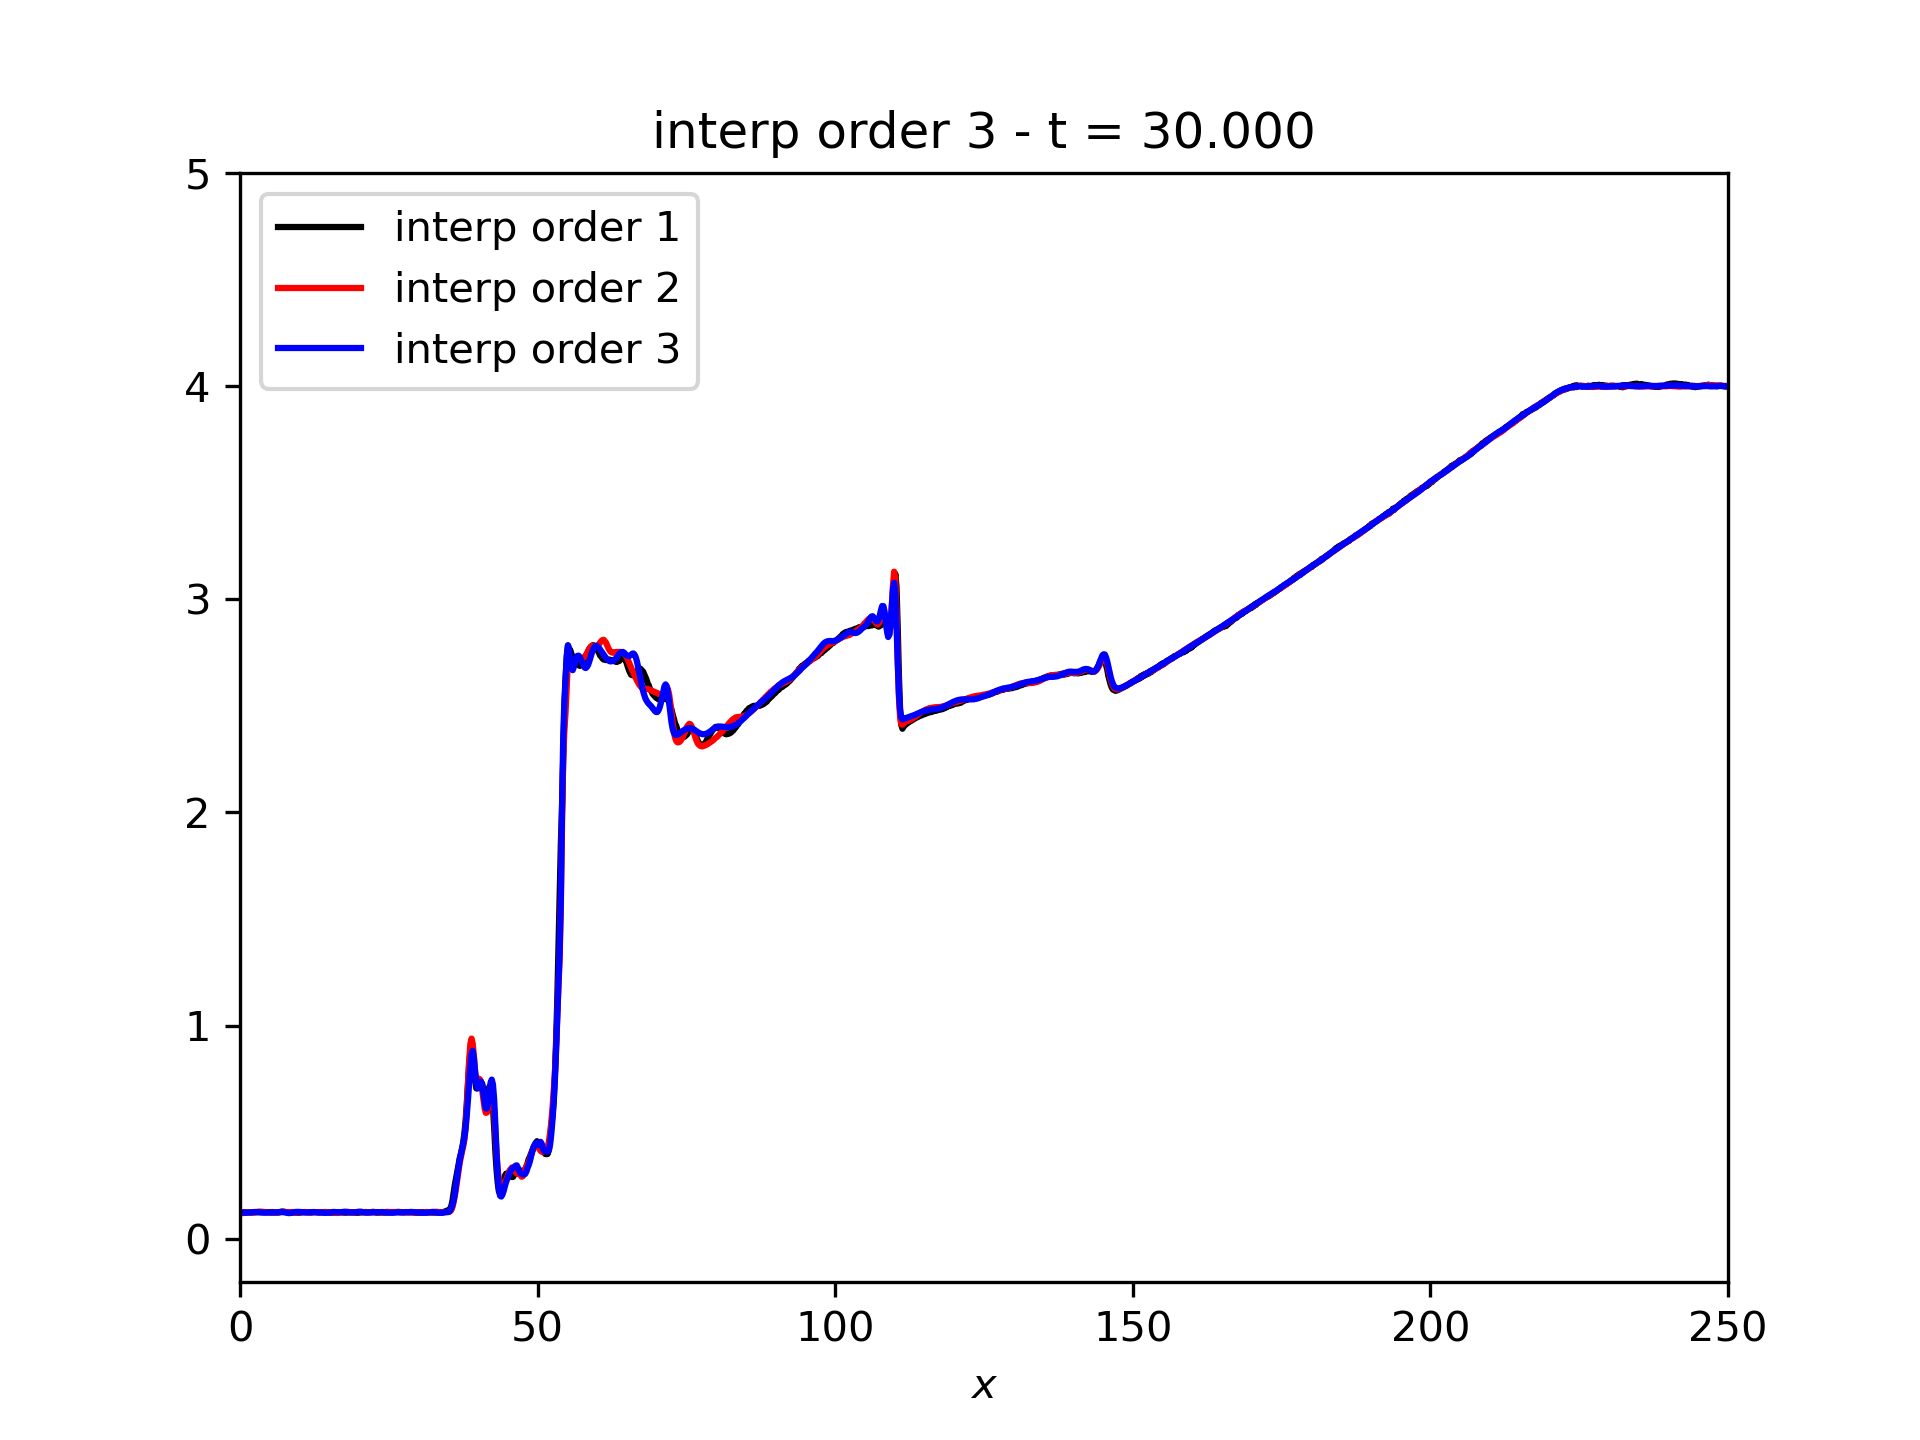
\includegraphics{shock/shock_By}
\caption{$B_y$ for different b-spline orders}
\label{fig:shock_bspline_order}
\end{figure}


\subsection{Role of the hyper-resistivity}

Here we look at the final time as a function of the hyper-resistivity value.


\begin{figure}[!t]
\centering
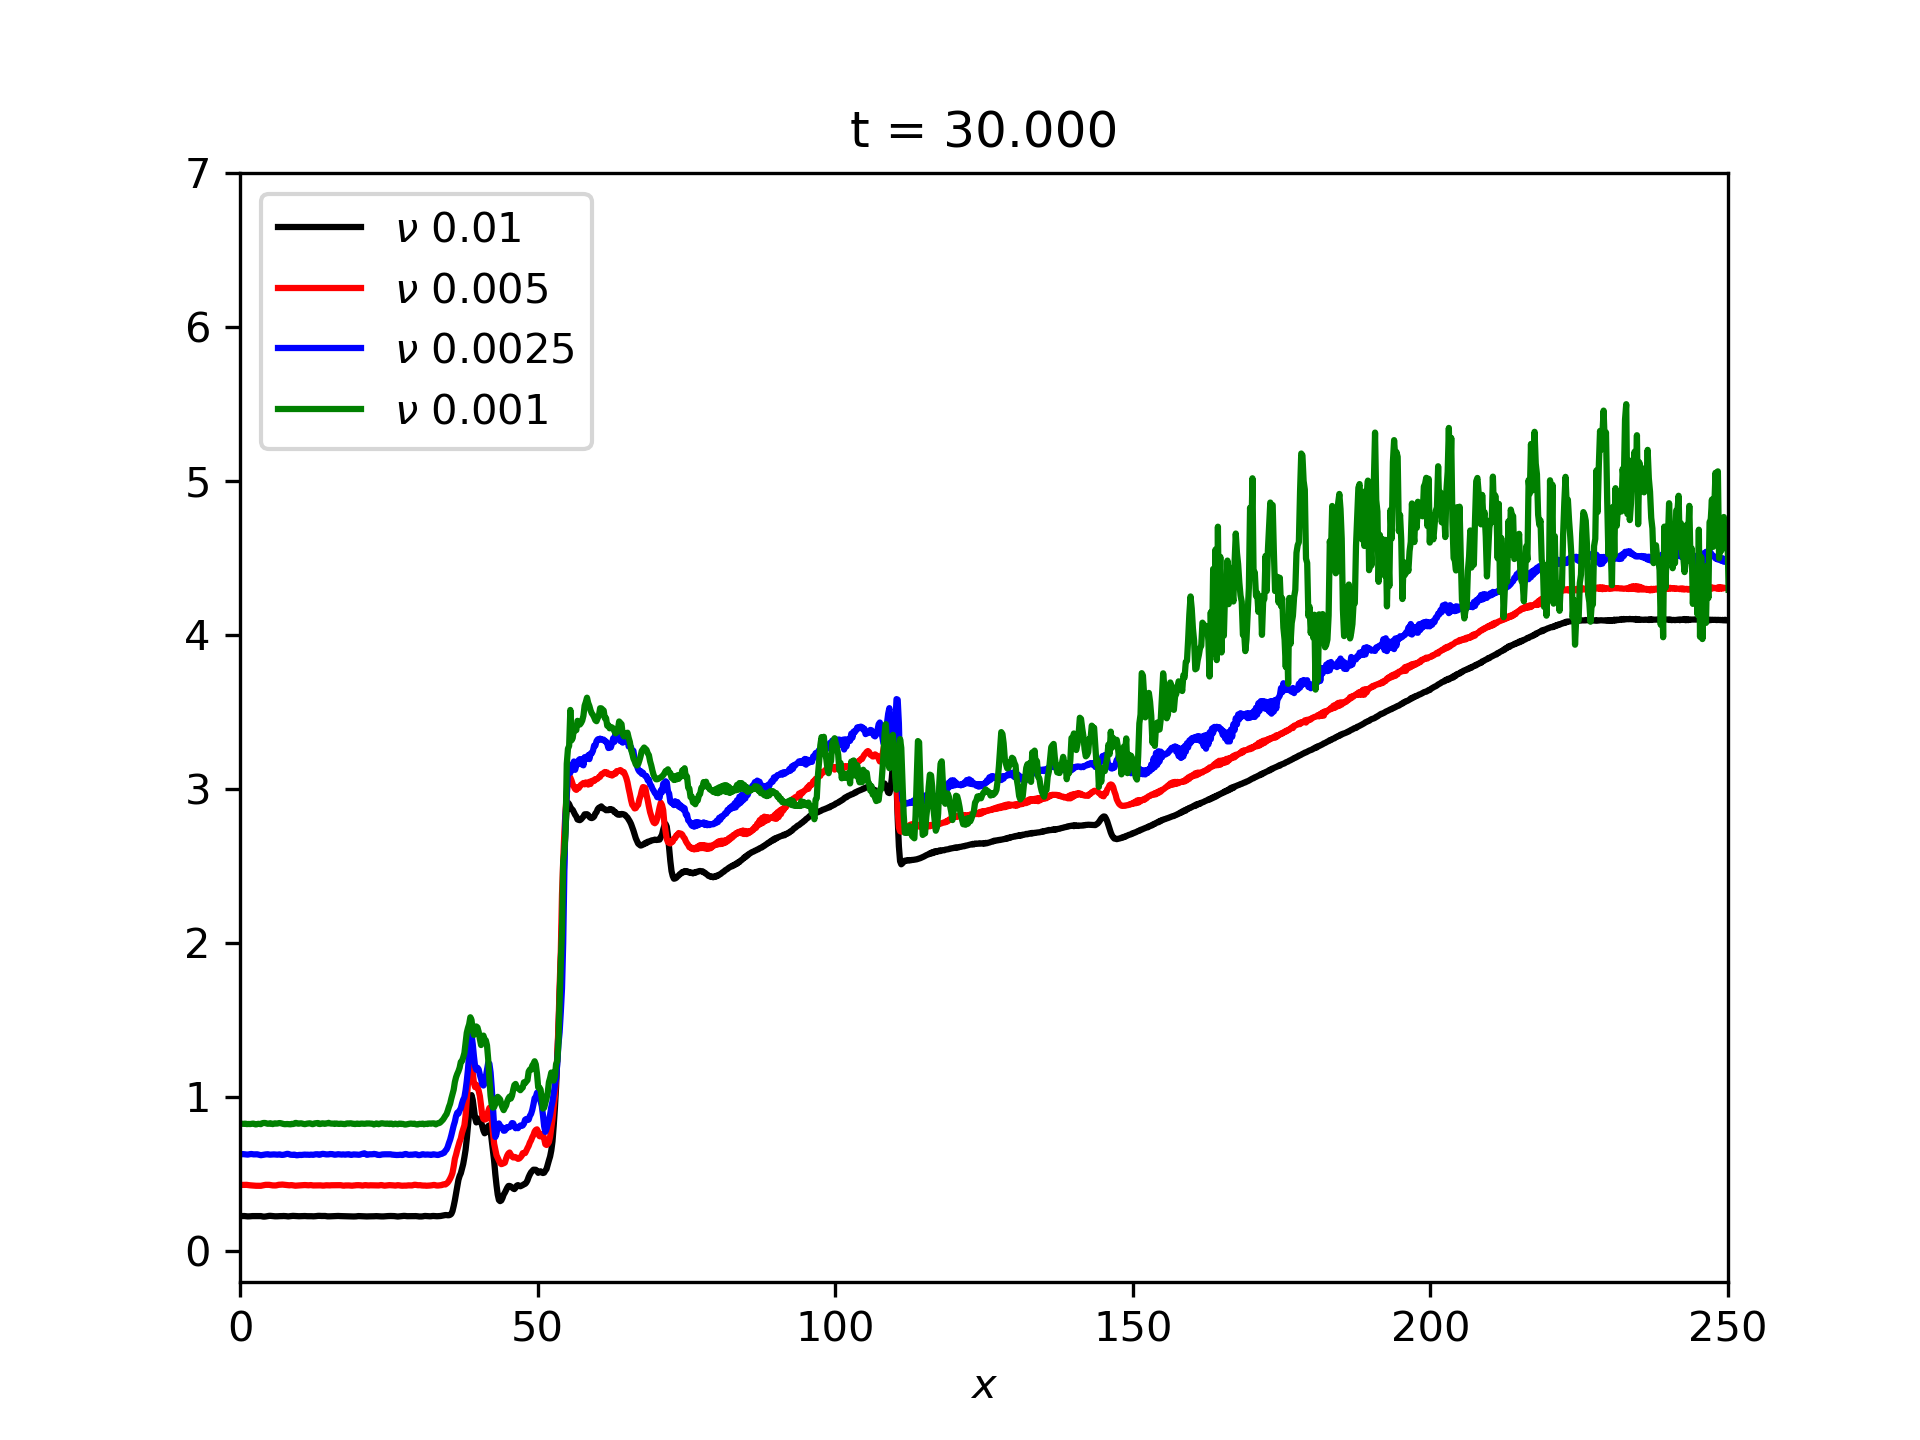
\includegraphics{shock/shock_By_nu}
\caption{$B_y$ for different values of $\nu$}
\label{fig:shock_bspline_order}
\end{figure}


